\DiaryEntry{Solving $x^n + \frac{1}{x^n} = 1$}{2016-02-09}{Maths}

This post is based on a problem in the Preface of the book ``Inside
Interesting Integrals''.

Consider the equation

\begin{equation}
\label{eq:n2}
x^n + \frac{1}{x^n} = 1
\end{equation}

with integer \(n\).

\subsubsection{Case \(n=1\)}

For \(n=1\) the solution is straightforward; we have

\[
x^2 + 1 = x \rightarrow x^2 - x + 1 = 0
\]

which has the two solutions

\[
x_{1,2} = \frac{1 \pm \sqrt{3}}{2} = e^{\pm j\pi/3}
\]

Note that the solution has an absolute value of \(1\) (as
\(\|e^{j \phi}\| = 1\)) and are shown in the Figure below.

\begin{figure}
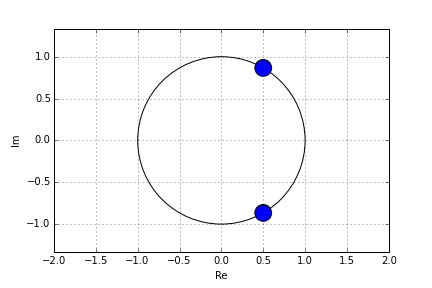
\includegraphics[scale=0.7]{images/complex_solutions.png}
\end{figure}

\subsubsection{Case \(n = 7\)}

For \(n = 7\), we have

\begin{equation}
\label{eq:n7}
x^7 + \frac{1}{x^7} = 1 \rightarrow x^{14} - x^7 + 1 = 0
\end{equation}

which we can solve with the substitution \(u=x^7\) and obtain

\[
u^2 - u + 1 = 0 \rightarrow u_{1,2} = \frac{1 \pm \sqrt{3}}{2} = e^{\pm j\pi/3}
\]

Now we need to solve for \(x\): We have \(u=e^{j\phi}\) and \(x^7 = u\),
therefore the (seven) solutions are

\[
x=e^{j\left( \frac{\phi}{7} + \frac{2\pi}{7}k\right)}\, ,\quad k=0,\ldots,6
\]

We have two solutions for \(u\); as each \(u\) solution become \(7\)
solutions for \(x\) we have in total 14 solutions for \(x\) - correct!

For \(u_1 = e^{j\pi/3}\), we have

\[
x_{1 \ldots 7} = e^{j\left( \frac{\pi}{21} + \frac{2\pi}{7}k\right)}\, ,\quad k=0,\ldots,6
\]

and for \(k=1\) the solution \(x_1\) is equal to \(u_1\). In a similar
spirit, we have for \(u_1 = e^{j\pi/3}\),

\[
x_{8 \ldots 14} = e^{j\left( -\frac{\pi}{21} + \frac{2\pi}{7}k\right)}\, ,\quad k=0,\ldots,6
\]

For \(k=6\), we obtain \(x_{13} = e^{j5\pi / 3}\) and this equals
\(u_2=e^{-j\pi/3} = e^{j5\pi / 3}\).

\textbf{Conclusion:} Equation \eqref{eq:n2} has the same solutions as
equation \eqref{eq:n7}. However, \eqref{eq:n7} has additional solutions
- in total 14 - as it is a polynomial of degree 14.
